\documentclass[11pt,a4paper]{article}
\usepackage[utf8]{inputenc}
\usepackage[margin=1in]{geometry}
\usepackage{amsmath}
\usepackage{amssymb}
\usepackage{amsthm}
\usepackage{graphicx}
\usepackage{hyperref}
\usepackage{xcolor}
\usepackage{natbib}
\usepackage{booktabs}
\usepackage{subcaption}

\hypersetup{
    colorlinks=true,
    linkcolor=blue,
    citecolor=blue,
    urlcolor=cyan,
}

\title{Not All Fillers Substitute for Reasoning: A Replication and Extension of
Filler-Token Experiments on Qwen3}
\author{ASI Research Lab\\
        \texttt{asi@cybergolem.ai}}
\date{November 25, 2026}

\begin{document}

\maketitle

\begin{abstract}
\citet{baherwani2026not} report that prefilled filler tokens---semantically
irrelevant sequences inserted before a model's answer---improve accuracy on
synthetic arithmetic, implying that some of a model's useful computation is
\emph{latent} and can be triggered by token bulk rather than problem-specific
content. Whether such latent computation can \emph{substitute} for explicit
chain-of-thought (CoT), or at least buy serving-side efficiency, has not been
quantified. We replicate the baseline filler experiment on
Qwen3-235B-A22B-Instruct-2507 and extend it along three axes: a direct
substitution test pitting a 200-token ASD-STE100 controlled-vocabulary filler
against full CoT, a hardware-grounded accounting of KV-cache memory and decode
costs, and a $2\times8\times2$ recovery grid sweeping model scale, filler length,
and CoT token budget. Our 10-shot replication is \emph{partial}: the original
multi-step arithmetic null ($-1.3$~pp) reproduces ($+0.57 \pm 1.63$~pp), whereas
the multiplication null ($-0.4$~pp) diverges ($+8.30 \pm 4.59$~pp), a shift we
attribute to FP8 endpoint quantization rather than prompting. Across our
extensions, filler computation is sharply bounded. Prefilling ${\sim}200$
ASD-STE100 tokens lifts 0-shot 4-digit multiplication from 34.2\% to 46.4\%
($+12.20 \pm 3.33$~pp, McNemar $p<10^{-11}$)---consistent with additional
parallel attention width---but recovers only ${\sim}19\%$ of the gap to full CoT
(97.2\%), and slightly \emph{degrades} sequential multi-step arithmetic
($-1.20 \pm 0.92$~pp). Shifting tokens from autoregressive decode to parallel
prefill cuts decode-stage KV token-reads by $78\times$--$170\times$ and
per-query wall clock by ${\sim}16\times$; however, the filler beats
budget-matched CoT only when CoT is capped below 512 tokens, a regime in which
CoT emits no final answer in 97--100\% of trials. Across the recovery grid,
filler gains peak at 200 tokens, vanish on a $7.7\times$ smaller Qwen3-30B-A3B
model (scale--filler cross-partial $+7.3 \pm 5.5$~pp per 100 tokens per parameter
decade), and are strictly Pareto-dominated by running full CoT on that smaller
model. Filler tokens surface only shallow, parallelizable latent computation in
high-capability models; they are not a substitute for serial reasoning.
\end{abstract}

\section{Introduction}

Chain-of-thought (CoT) prompting \citep{wei2022cot} improves language-model
reasoning for two entangled reasons. It lets the model externalise intermediate
symbolic states into the token stream, and it simply grants the transformer more
forward-pass token positions over which to route hidden attention computation
\citep{pfau2024dot,goyal2024pause}. Separating these mechanisms matters for both
AI safety and inference systems. From a safety perspective,
\citet{baherwani2026not} show that inserting a fixed, semantically irrelevant
\emph{filler} sequence before the answer cue of a no-CoT prompt raises accuracy
on synthetic tasks for several frontier models, which means consequential
``invisible reasoning'' can occur without an auditable text trace. From a systems
perspective, prefilled filler tokens are processed in a single parallel,
compute-bound pass rather than sequential, memory-bandwidth-bound autoregressive
decoding---raising the prospect of trading expensive CoT generation for cheap
prefill bulk.

Both implications hinge on a quantitative question that baseline comparisons
leave open: \emph{how much of explicit reasoning can prefilled fillers actually
replace, and under what capability and budget regimes?} In this paper we
replicate the baseline filler evaluation of \citet{baherwani2026not} on
Qwen3-235B-A22B-Instruct-2507 via OpenRouter \citep{openrouter2026} and extend it
across three progressively broader experiments.

First, we benchmark a prefilled filler directly against unconstrained 0-shot CoT.
We use an ASD-STE100 Simplified Technical English vocabulary filler rather than
the original counting sequence, for two reasons: counting fillers share surface
tokens (digits) with arithmetic problems, which confounds a lexical-interference
explanation with a compute explanation; and a controlled technical vocabulary is
semantically inert in a different way, so a positive result cannot be attributed
to the filler supplying task-relevant content. Our extensions then run 0-shot,
whereas the replication runs 10-shot, because in-context exemplars give the model
an explicit answer format and a partial worked method, and we want the
substitution test to isolate what the prefill itself contributes.

Second, given that fillers fall far short of full CoT accuracy, we invert the
hypothesis and ask an efficiency question: how much KV-cache footprint and decode
bandwidth do prefilled fillers save, and what is the marginal accuracy cost of
those savings?

Third, we map the accuracy--cost surface across three recovery axes---model scale
(235B-A22B vs.\ 30B-A3B), filler length (0--500 tokens), and CoT generation cap
(128--2048 tokens)---to locate where filler computation saturates and where
budget-capped CoT collapses.

Our contributions are fourfold.
\begin{enumerate}
    \item \textbf{Partial replication and serving-path diagnosis}
    (Section~\ref{sec:replication}). At 10-shot ($N{=}1000$ per cell), Qwen3-235B
    reproduces the original arithmetic null ($+0.57 \pm 1.63$~pp) but yields a
    positive multiplication gain ($+8.30 \pm 4.59$~pp against $-0.4$~pp
    reported); prompt ablations and uncached re-queries isolate FP8 endpoint
    quantization as the leading candidate for the shifted base rate.
    \item \textbf{A substitution bound against CoT} (Section~\ref{sec:stecot}).
    At 0-shot, a 200-token ASD-STE100 filler recovers ${\sim}19\%$ of the
    baseline-to-CoT gap on 4-digit multiplication and slightly harms multi-step
    arithmetic, consistent with limits on parallel versus serial transformer
    computation.
    \item \textbf{Prefill--decode KV accounting} (Section~\ref{sec:kv}). We
    formalise per-query peak KV memory, decode-stage KV token-reads, and KV
    occupancy, showing a $78\times$--$170\times$ read reduction and ${\sim}16\times$
    wall-clock reduction for the filler, at a steep accuracy price.
    \item \textbf{Multi-axis recovery and truncation-cliff analysis}
    (Section~\ref{sec:grid}). Across $2\times8\times2$ conditions we track explicit
    answer-cue rates to show that CoT collapses below 512 tokens, that filler
    gains follow an inverted U peaking at 200 tokens only on the 235B model, and
    that a 30B-A3B model with full CoT dominates the accuracy--memory Pareto
    frontier.
\end{enumerate}

\section{Background and Related Work}
\label{sec:related}

\subsection{Latent computation, pause tokens, and expressivity limits}

A growing body of work asks whether transformers can perform extra computation
across semantically empty token positions without externalising intermediate
steps in natural language. \citet{goyal2024pause} introduce learnable
\emph{pause} tokens appended during both pretraining and fine-tuning, and show
that delaying next-token prediction improves downstream reasoning when the model
is explicitly trained to exploit the extra width. \citet{pfau2024dot}
characterise the theoretical boundary of the mechanism: filler tokens such as
repeated dots expand parallel circuit width within constant-depth threshold
circuits ($\mathsf{TC}^0$), letting transformers solve parallelisable
combinatorial tasks without visible reasoning, whereas inherently sequential
problems still require routing intermediate states through emitted CoT tokens.
This distinction is the organising hypothesis of our results: it predicts that a
filler should help a task whose sub-results can be aggregated in parallel
(4-digit multiplication) and should not help one whose intermediate state must be
carried and updated serially (nested multi-step arithmetic). Our grid tests that
prediction directly.

Moving from custom-trained models to off-the-shelf frontier APIs,
\citet{baherwani2026not} test whether pretrained models already exhibit invisible
reasoning when fixed filler sequences (counting numbers, repeated characters, or
random words) are prefilled between the question and the answer cue of a $K$-shot
no-CoT prompt. Across 13 frontier models they observe gains of up to 13~pp, with
strong model and token dependence: for Qwen3-235B-A22B they report 10-shot nulls
on both multiplication ($69.6\%\to69.2\%$, $\Delta=-0.4$~pp) and multi-step
arithmetic ($11.0\%\to9.7\%$, $\Delta=-1.3$~pp), a modest 0-shot multiplication
lift ($57.3\%\to60.9\%$, $+3.6$~pp; their Appendix Table~10), and no benefit when
baseline capability is near zero (their Appendix~B.2). They compare fillers
against a no-CoT baseline, which establishes the \emph{existence} of invisible
computation. We compare fillers against full and budget-capped CoT, which
establishes its \emph{ceiling}.

\subsection{Inference-time token budgets and serving asymmetry}

Explicit CoT reliably unlocks multi-digit arithmetic and symbolic manipulation
\citep{wei2022cot}, but autoregressive decoding is memory-bandwidth-bound: every
generated token re-reads the entire growing key--value (KV) cache. Work on
adaptive test-time compute \citep{damani2025learning} learns policies that
allocate generation budgets across queries according to predicted difficulty.
Our setting is different in a way that matters for measurement: rather than
learning an allocation policy, we impose a hard cap on a fixed instruction model.
If a derivation exceeds the cap, generation terminates before the answer cue, and
any parser that reads the last number in the trace will score an intermediate
sub-result. Section~\ref{sec:trunc} makes that failure mode measurable instead of
silent, which is what allows us to separate genuine efficiency from truncation
artefacts.

\section{Methodology}
\label{sec:method}

Our aim is to measure, on identical problems, what prefilled filler tokens buy
relative to (i) no computation at all and (ii) explicit reasoning, and at what
serving cost. We therefore hold the problem set fixed across every condition and
vary only the prompt and the decode budget.

\subsection{Tasks, models, and serving}

Following Section~3.2 and Appendix~A.2 of \citet{baherwani2026not}, we evaluate
two synthetic benchmarks chosen for their differing computational structure.
\textbf{4-digit multiplication} ($a\times b$ with $a,b\in[1000,9999]$) admits a
decomposition into partial products that can in principle be formed and
aggregated in parallel. \textbf{Left-nested multi-step arithmetic} comprises five
sequential binary operations with operands $|x|\geq100$ and answers of at least
seven digits; because each operation consumes the previous result, the
intermediate state must be carried and updated serially. Each cell evaluates
$N{=}1000$ problems drawn from fixed seeds (\texttt{12345} and \texttt{54321}),
so every condition and every model sees identical inputs and paired comparisons
are exact.

We evaluate two Mixture-of-Experts models from the non-thinking Qwen3-2507
instruction family: \texttt{qwen/qwen3-\allowbreak235b-\allowbreak a22b-\allowbreak2507} (235B total, 22B active
parameters) and \texttt{qwen/qwen3-\allowbreak30b-\allowbreak a3b-\allowbreak instruct-\allowbreak2507} (30.5B total, 3.3B
active). Both are served through OpenRouter \citep{openrouter2026} at temperature
$1.0$ and top-$p$ $0.95$, with internal thinking disabled on all no-CoT
conditions. Our harness caches each raw response under a hash of the exact JSON
request body, which makes replay free and guarantees that a rerun cannot silently
change a condition; Section~\ref{sec:stats} exploits that property to recover
per-problem outcomes for all 1000 items per cell.

\subsection{Prompting and budget conditions}

Beyond the 10-shot replication of the original numeric \textbf{counting} filler
(Section~\ref{sec:replication}), our 0-shot extensions compare eight conditions
designed to separate prefill length from autoregressive budget.
\begin{itemize}
    \item \textbf{baseline}: a no-CoT prompt whose assistant turn is prefilled up
    to the literal answer cue, with no filler tokens. This is the floor against
    which filler uplift is measured.
    \item \textbf{ste\_filler} ($L_{\mathrm{STE}}{=}200$): a fixed sequence of
    words drawn from the ASD-STE100 Simplified Technical English controlled
    vocabulary, prefilled before the answer cue and identical across all queries
    (Appendix~\ref{app:filler}). Its length is calibrated to 199 \texttt{o200k}
    tokens locally; the Qwen tokenizer segments the same string into ${\sim}202$
    tokens, and the ${\sim}1.5\%$ difference is ordinary BPE vocabulary
    mismatch rather than a configuration error.
    \item \textbf{ste\_100} and \textbf{ste\_500}: the same construction
    calibrated to 100 and 500 tokens, to measure length sensitivity and
    saturation.
    \item \textbf{cot} (\textbf{CoT 2048}): an unconstrained 0-shot reasoning
    prompt instructing the model to solve step by step and finish with
    \texttt{Answer: [ANSWER]} (\texttt{max\_tokens}${=}2048$), scored by a parser
    anchored on the final \texttt{Answer:} cue.
    \item \textbf{cot\_128}, \textbf{cot\_256}, \textbf{cot\_512}: identical to
    \textbf{cot} but capped at 128, 256, or 512 tokens, to trace accuracy under
    strict decode budgets.
\end{itemize}

\subsection{Truncation measurement}
\label{sec:trunc}

A token-capped CoT trace that hits \texttt{max\_tokens} mid-calculation still
contains intermediate numbers, so a last-number fallback parser extracts an
unfinished sub-result and registers an apparent reasoning error. To separate a
wrong answer from an unfinished derivation we record the \emph{explicit answer-cue
rate}: the fraction of completions containing the literal string \texttt{Answer:}.
For CoT conditions $1-\text{explicit rate}$ is the mid-derivation truncation rate.
For no-CoT conditions the cue resides in the assistant prefill, so the metric is
not informative there and we do not report it as a truncation measure.

\subsection{KV-cache accounting}
\label{sec:kvacct}

To compare serving cost between prefill-heavy fillers and decode-heavy CoT we
model per-query KV demand from the API-reported prompt tokens $T_p$ and
completion tokens $T_c$. Peak KV footprint is proportional to $T_p+T_c$. Because
decoding is memory-bandwidth-bound, each sequential step $t\in\{0,\dots,T_c-1\}$
must read all preceding KV entries, so decode-stage KV token-reads are
\begin{equation}
\label{eq:reads}
R_{\mathrm{KV}} \;=\; \sum_{t=0}^{T_c-1}(T_p+t)
\;=\; T_cT_p+\tfrac{1}{2}T_c(T_c-1),
\end{equation}
and KV \emph{occupancy}---the time integral of resident KV---is
$T_{\mathrm{KV}}\cdot$ wall-clock per query. Under \texttt{bf16} storage
(2~bytes per element, key and value) Qwen3-235B (94 layers, 4 KV heads, head
dimension 128) needs $2\times94\times4\times128\times2=192{,}512$~B
(${\sim}188$~KiB) per token, and Qwen3-30B (48 layers) needs 96~KiB.
Equation~\eqref{eq:reads} exposes the asymmetry that motivates the filler:
tokens placed in $T_p$ contribute linearly through $T_cT_p$ when the answer is
short, whereas tokens generated into $T_c$ incur the quadratic
$\mathcal{O}(T_c^2)$ term.

\subsection{Statistical tests}
\label{sec:stats}

Cell accuracies ($N{=}1000$) carry 95\% binomial intervals. Condition
differences are measured on paired per-problem outcomes. The harness's response
cache retains every completion, and the task generator and filler calibration are
deterministic, so we can rebuild each request body and recover the outcome of all
1000 problems per cell; we verified this reconstruction against the cache with
zero misses across all 32 cells. Paired deltas therefore use the full $N{=}1000$,
with exact one-sided McNemar tests and paired $t$-intervals. Finite-difference
slopes across the grid propagate cell standard errors in quadrature.

\section{Results}
\label{sec:results}

\subsection{Replication: 10-shot baseline versus counting filler}
\label{sec:replication}

We first ask whether the 10-shot nulls that \citet{baherwani2026not} report for
Qwen3-235B-A22B hold under live OpenRouter serving (Table~\ref{tab:replication},
$N{=}1000$ per cell). The replication splits cleanly by task. On multi-step
arithmetic the original null reproduces: we measure $+0.57 \pm 1.63$~pp against
their $-1.3$~pp. On 4-digit multiplication, where they found no effect
($-0.4$~pp from a 69.6\% baseline), we measure a significant
$+8.30 \pm 4.59$~pp lift from a depressed 58.70\% baseline. The filler raises
accuracy to 67.00\%, close to the 69.2\% the original study obtained \emph{without}
a filler.

\begin{table}[h]
\centering
\caption{Replication of the 10-shot baseline-versus-counting experiment
($N{=}1000$ per cell). Paper values from \citet{baherwani2026not}, Table~1.}
\label{tab:replication}
\begin{tabular}{llcc}
\toprule
\textbf{Task} & \textbf{Condition} & \textbf{Paper} & \textbf{Ours} \\
\midrule
Multiplication & baseline & 69.6 & 58.70 \\
Multiplication & counting & 69.2 & 67.00 \\
Multiplication & $\Delta$ & $-0.4$ & $\mathbf{+8.30 \pm 4.59}$ \\
\midrule
Arithmetic & baseline & 11.0 & 6.25 \\
Arithmetic & counting & 9.7 & 6.82 \\
Arithmetic & $\Delta$ & $-1.3$ & $+0.57 \pm 1.63$ \\
\bottomrule
\end{tabular}
\end{table}

Our baselines sit 10.9~pp (multiplication) and 4.75~pp (arithmetic) below the
original. To test whether prompt formatting or caching caused the shift we ran
two $N{=}1000$ ablations---0-shot prompting, and a minimal \texttt{/no\_think}
system directive---followed by uncached live re-queries; none closed the gap.
Inspection of provider metadata then showed a concrete infrastructure difference:
every endpoint serving this model during our runs operated in FP8 precision,
whereas the serving precision of the original study is unspecified. The pattern
is consistent with quantization degrading single-pass partial-product arithmetic,
leaving headroom that extra attention passes over filler positions can partially
recover: the filler restores accuracy to nearly the original ceiling rather than
exceeding it.

\subsection{Extension 1: ASD-STE100 filler versus full CoT}
\label{sec:stecot}

Establishing that a filler beats a no-CoT prompt does not establish that it
substitutes for reasoning. We therefore move to a clean 0-shot setting without
in-context exemplars and ask whether a 200-token controlled-vocabulary filler can
close the gap to unconstrained CoT (Table~\ref{tab:stecot},
Figure~\ref{fig:stecot}).

\begin{table}[h]
\centering
\caption{ASD-STE100 filler versus full CoT, 0-shot, $N{=}1000$
(Qwen3-235B-A22B-2507). All $\Delta$ values are paired over the same 1000
problems; intervals are 95\% paired $t$-intervals.}
\label{tab:stecot}
\begin{tabular}{lccc}
\toprule
\textbf{Task} & \textbf{Condition} & \textbf{Accuracy (\%)} & $\mathbf{\Delta}$ \textbf{vs.\ CoT} \\
\midrule
Multiplication & baseline & $34.20 \pm 2.94$ & $-63.00 \pm 3.13$ \\
Multiplication & ste\_filler & $46.40 \pm 3.09$ & $\mathbf{-50.80 \pm 3.26}$ \\
Multiplication & CoT & $97.20 \pm 1.02$ & --- \\
\midrule
Arithmetic & baseline & $4.27 \pm 1.29$ & $-92.50 \pm 1.68$ \\
Arithmetic & ste\_filler & $2.84 \pm 1.04$ & $\mathbf{-93.70 \pm 1.53}$ \\
Arithmetic & CoT & $96.50 \pm 1.14$ & --- \\
\bottomrule
\end{tabular}
\end{table}

\begin{figure}[t]
    \centering
    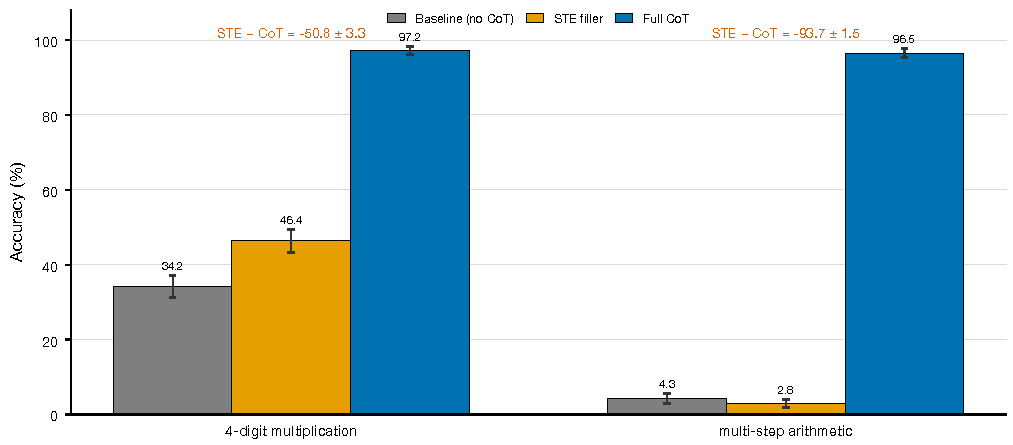
\includegraphics[width=\textwidth]{figs/ste-vs-cot.pdf}
    \caption{0-shot accuracy by condition (Qwen3-235B-A22B-2507, $N{=}1000$).
    The controlled-vocabulary filler buys a partial uplift on multiplication and
    a small regression on arithmetic, while full CoT saturates both. Bars are
    95\% binomial intervals.}
    \label{fig:stecot}
\end{figure}

The results expose a boundary governed by task seriality. On multiplication the
filler lifts accuracy by $+12.20 \pm 3.33$~pp over baseline
($34.20\%\to46.40\%$), recovering ${\sim}19\%$ of the 63.0~pp deficit to full CoT,
but still trailing CoT by $50.80 \pm 3.26$~pp on paired problems. On nested
arithmetic the same filler provides no benefit and trends slightly below baseline
($2.84\%$ vs.\ $4.27\%$, $-1.20 \pm 0.92$~pp, McNemar $p=0.998$ for any positive
effect), trailing CoT by $93.70 \pm 1.53$~pp. The paired discordant counts are
lopsided in the same direction: on multiplication CoT is correct where the filler
fails on 521 problems against 13 in the reverse direction; on arithmetic the split
is 938 to 1.

That asymmetry is what the $\mathsf{TC}^0$ account predicts. Multiplication's
partial products can be formed and combined by a wide, shallow circuit that extra
token positions make room for; a five-step nested expression requires the
intermediate value to be written, read back, and updated in order, which is the
serial depth that CoT supplies and a prefill does not. The filler is therefore
buying parallel width, not reasoning.

\subsection{Extension 2: the efficiency inversion}
\label{sec:kv}

Because the filler cannot match CoT accuracy, the natural systems question is
whether it nonetheless offers a compelling low-latency operating point. We test
the inverted null hypothesis $H_0$: prefilled fillers provide no KV-cache memory
or decode-bandwidth saving over CoT.

Equation~\eqref{eq:reads} on our 0-shot runs rejects $H_0$ decisively
(Table~\ref{tab:kv}, Figure~\ref{fig:kvtradeoff}). Moving ${\sim}202$ tokens into
the assistant prefill leaves answer generation short ($T_c\approx7$--$11$ tokens),
whereas full CoT generates 630--758 tokens sequentially. The filler consequently
needs $78\times$ (multiplication) and $170\times$ (arithmetic) fewer decode-stage
KV token-reads than CoT, occupies $0.42\times$ and $0.37\times$ of CoT's peak KV,
cuts KV occupancy by $37\times$ and $46\times$, and reduces amortised per-query
wall clock by ${\sim}15$--$16\times$.

The saving comes with two caveats that Table~\ref{tab:kv} makes explicit. First,
relative to \emph{baseline} rather than CoT the filler is more expensive, not
less: it costs $3.2\times$ the peak KV and $3.6\times$ the decode reads for a
$1.5\times$ wall-clock penalty, because it adds 202 prompt tokens to a query whose
answer was already short. Second, the accuracy exchange rate against CoT is steep:
each $1\times$ reduction in decode reads costs $0.66$~pp of accuracy on
multiplication and $0.56$~pp on arithmetic. Whether that trade is ever
Pareto-efficient depends on how CoT behaves under matched caps, which is the next
question.

\begin{table}[t]
\centering
\caption{Per-query KV and latency accounting (Qwen3-235B, 0-shot, $N{=}1000$).
$T_p$ and $T_c$ are mean API prompt and completion tokens; $R_{\mathrm{KV}}$ is
Eq.~\eqref{eq:reads}; peak KV assumes uncached \texttt{bf16} storage at
188~KiB/token; \emph{unshared} is the KV left after the static prefix is cached
once; occupancy is $T_{\mathrm{KV}}\cdot$ wall clock.}
\label{tab:kv}
\small
\begin{tabular}{llrrrrrr}
\toprule
\textbf{Task} & \textbf{Cond.} & $T_p$ & $T_c$ & $R_{\mathrm{KV}}$ &
\textbf{Peak MiB} & \textbf{Unshared} & \textbf{Occ.\ MB$\cdot$s} \\
\midrule
Mult. & baseline & 80.4 & 10.3 & 873 & 16.7 & 20.3 & 1.3 \\
Mult. & ste\_filler & 282.5 & 10.9 & 3{,}118 & 53.9 & 20.8 & 6.2 \\
Mult. & CoT & 70.0 & 630.4 & 242{,}483 & 128.6 & 640.4 & 232.0 \\
\midrule
Arith. & baseline & 99.7 & 7.9 & 810 & 19.8 & 35.0 & 1.7 \\
Arith. & ste\_filler & 301.9 & 6.9 & 2{,}089 & 56.7 & 34.0 & 7.1 \\
Arith. & CoT & 89.4 & 757.5 & 354{,}229 & 155.5 & 784.6 & 327.0 \\
\bottomrule
\end{tabular}
\end{table}

\begin{figure}[t]
    \centering
    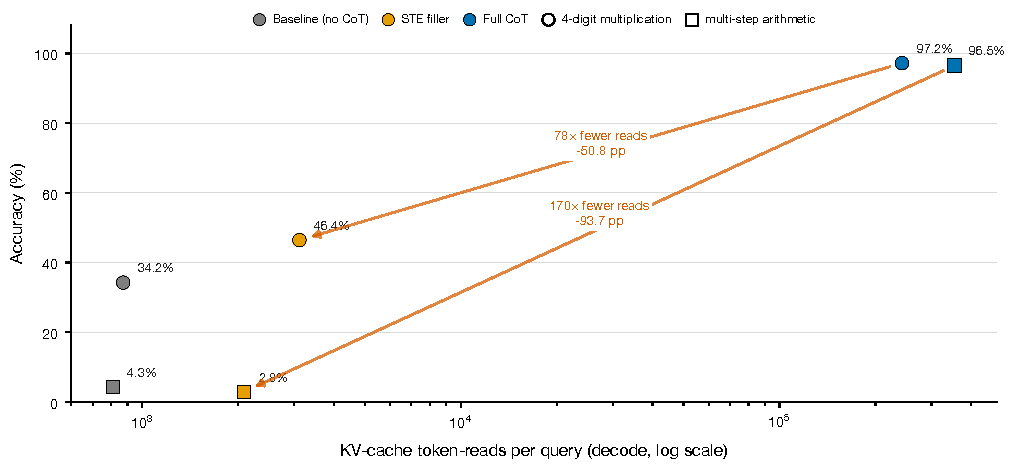
\includegraphics[width=\textwidth]{figs/kv-tradeoff.pdf}
    \caption{Accuracy against decode-stage KV token-reads (log scale). Arrows run
    from full CoT to the STE filler: $78\times$ and $170\times$ fewer reads at a
    cost of 50.8 and 93.7~pp of accuracy.}
    \label{fig:kvtradeoff}
\end{figure}

\subsection{Extension 3: the recovery grid}
\label{sec:grid}

Comparing a single 200-token filler on one model against unconstrained CoT
conflates token budget with reasoning mode and leaves model scale unexplored. To
map the whole surface we evaluate a $2\times8\times2$ grid
($N{=}1000$ per cell, Table~\ref{tab:grid}) over filler length
$\{0,100,200,500\}$, CoT cap $\{128,256,512,2048\}$, and model
$\{$235B-A22B, 30B-A3B$\}$. Four structural findings emerge.

\begin{table}[t]
\centering
\caption{Recovery grid: accuracy (\%) $\pm$ 95\% binomial interval, 0-shot,
$N{=}1000$ per cell. Bold marks the best condition in each row.}
\label{tab:grid}
\resizebox{\textwidth}{!}{
\begin{tabular}{llcccccccc}
\toprule
\textbf{Model} & \textbf{Task} & \textbf{base} & \textbf{STE 100} &
\textbf{STE 200} & \textbf{STE 500} & \textbf{CoT 128} & \textbf{CoT 256} &
\textbf{CoT 512} & \textbf{CoT 2048} \\
\midrule
235B & mult & $34.2{\pm}2.9$ & $40.7{\pm}3.0$ & $\mathbf{46.4{\pm}3.1}^{\dagger}$ & $43.4{\pm}3.1$ & $0.0$ & $0.9{\pm}0.6$ & $60.8{\pm}3.0$ & $97.2{\pm}1.0$ \\
235B & arith & $\mathbf{4.3{\pm}1.3}$ & $3.0{\pm}1.1$ & $2.8{\pm}1.0$ & $3.5{\pm}1.1$ & $0.0$ & $1.8{\pm}0.8$ & $37.2{\pm}3.0$ & $96.5{\pm}1.1$ \\
30B & mult & $8.3{\pm}1.7$ & $8.3{\pm}1.7$ & $8.8{\pm}1.8$ & $7.6{\pm}1.6$ & $0.0$ & $1.2{\pm}0.7$ & $68.8{\pm}2.9$ & $\mathbf{98.6{\pm}0.7}$ \\
30B & arith & $3.2{\pm}1.2$ & $2.4{\pm}1.0$ & $2.2{\pm}0.9$ & $2.3{\pm}1.0$ & $0.0$ & $3.5{\pm}1.1$ & $42.7{\pm}3.1$ & $\mathbf{94.0{\pm}1.5}$ \\
\bottomrule
\end{tabular}
}
\smallskip
{\footnotesize $^{\dagger}$Best no-CoT condition; full CoT is best overall. Zero
cells show $\pm0.00$ because all 1000 traces truncated identically.}
\end{table}

\paragraph{CoT is a cliff, not a curve.}
Accuracy does not degrade gracefully as the cap tightens; it collapses below 512
tokens on both models (Table~\ref{tab:grid}, Figure~\ref{fig:sensitivity}b). On
the 235B model the explicit answer-cue rates at caps 128, 256, 512 and 2048 are
$0.1\%,0.9\%,60.8\%,97.8\%$ on multiplication ($0.0\%,1.7\%,36.4\%,97.4\%$ on
arithmetic), tracking cell accuracy almost one-for-one. Below 512 tokens the model
exhausts its budget mid-derivation, and the fallback parser scores a partial
product: the near-zero accuracy is an absent answer, not a wrong one. Marginal CoT
return therefore jumps from under 1~pp per 100 tokens on $[128,256]$ to
$+23.4$~pp per 100 tokens on $[256,512]$ for 235B multiplication.

\paragraph{Filler gains saturate, then reverse.}
If prefilled tokens were general-purpose serial compute, lengthening the filler
should keep closing the gap to CoT. Instead the marginal gains on 235B
multiplication across $[0,100]$, $[100,200]$ and $[200,500]$ are $+6.5$, $+5.7$
and $-1.0$~pp per 100 tokens (Figure~\ref{fig:sensitivity}a): an inverted U that a
quadratic captures ($R^2=0.99$) and a line does not ($R^2=0.39$). A plausible
reading is positional dilution, where attention between the question and the
answer cue is spread over more inert positions past 200 tokens. On arithmetic, and
on the 30B model for both tasks, every interval is indistinguishable from zero.

\paragraph{Model size buys accuracy only without CoT.}
Scaling from 30.5B to 235B parameters (0.887 decades) strongly lifts no-CoT
multiplication ($\partial\mathrm{Acc}/\partial\log_{10}N_{\mathrm{total}}
=+29.2\pm3.8$~pp per decade, or $+1.27\pm0.17$~pp per 10B total and
$+13.9\pm1.8$~pp per 10B active; Figure~\ref{fig:sensitivity}c). Under full CoT
the same derivative vanishes ($-1.6\pm1.4$~pp per decade) and the 30B model
matches or edges out the 235B ($98.6\%$ vs.\ $97.2\%$). Parameter scale
compensates for missing scratchpad tokens in single-pass inference, and adds
nothing once the steps are externalised.

\paragraph{Scale and filler length are complements.}
Taking increasing $N_{\mathrm{total}}$ as positive, the mixed second difference
$\partial^2\mathrm{Acc}/\partial\log_{10}N_{\mathrm{total}}\,\partial L_{\mathrm{STE}}$
on multiplication is $+7.3\pm5.5$ and $+5.9\pm5.6$~pp per 100 tokens per decade
over $[0,100]$ and $[100,200]$: the 235B model converts filler tokens into
accuracy at roughly $+6.5$ and $+5.7$~pp per 100, while the 30B converts
$+0.0$ and $+0.5$. (The sign follows from increasing $N$; reading the slope
difference in the opposite direction reverses it, which is why we state the
convention explicitly.) Only a model with substantial single-pass capability
($34.2\%$ baseline versus $8.3\%$) has latent circuits mature enough for filler
positions to amplify, which quantifies the capability precondition that
\citet{baherwani2026not} note qualitatively in their Appendix~B.2.

\paragraph{The Pareto frontier is the small model with full CoT.}
Plotting accuracy against KV cost (Figure~\ref{fig:pareto}) shows why fixed-budget
comparisons mislead. Around 54--63~MiB of peak KV on the 235B model,
\texttt{ste\_filler} (46.4\%) appears to beat \texttt{cot\_256} (0.9\%) by
45.5~pp---but \texttt{cot\_256} fails to emit an answer in 99.1\% of trials. At
the first cap where CoT usually finishes, \texttt{cot\_512} reaches 60.8\% and
overtakes even \texttt{ste\_500} (43.4\%). The global frontier point is
\textbf{Qwen3-30B-A3B with full CoT}: 98.6\% multiplication accuracy inside a
53.1~MiB peak KV footprint, matching the memory budget of 235B
\texttt{ste\_filler} (53.9~MiB) at $+52.2$~pp higher accuracy. Comparing
marginal slopes on 235B multiplication gives an effective marginal rate of
technical substitution
$\mathrm{MRTS}_{L_{\mathrm{STE}},L_{\mathrm{CoT}}}=0.78$ CoT tokens per STE
token (95\% CI 0.43--1.16), computed as the ratio of
$\partial\mathrm{Acc}/\partial L_{\mathrm{STE}}$ averaged over the full
$[0,500]$ range ($+1.84$~pp per 100) to
$\partial\mathrm{Acc}/\partial L_{\mathrm{CoT}}$ over $[512,2048]$
($+2.37$~pp per 100), with a parametric bootstrap over the two slope standard
errors. It is a global average ratio, not a local derivative at a single point.
Even where fillers work best, each prefilled token buys less than one token of
explicit reasoning.

\begin{figure}[t]
    \centering
    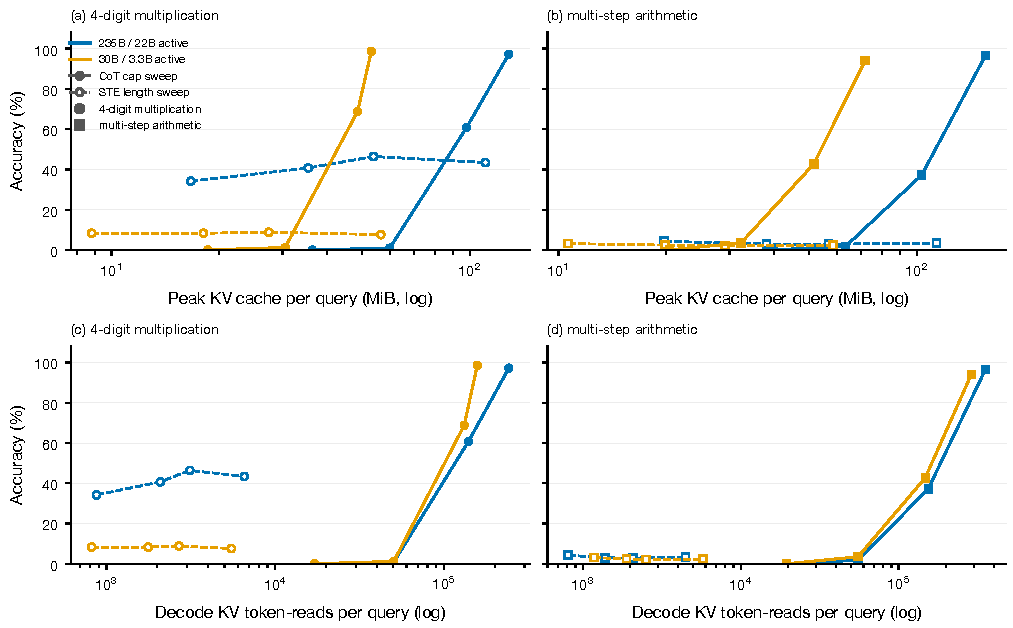
\includegraphics[width=\textwidth]{figs/recovery-pareto.pdf}
    \caption{Accuracy against peak KV memory (top) and decode-stage KV
    token-reads (bottom), both log scale, across models and tasks. Dashed curves
    sweep STE filler length (0--500); solid curves sweep CoT caps (128--2048).
    Truncated CoT sits near zero below ${\sim}50$~MiB and then climbs steeply;
    30B with full CoT dominates the peak-KV frontier.}
    \label{fig:pareto}
\end{figure}

\begin{figure}[t]
    \centering
    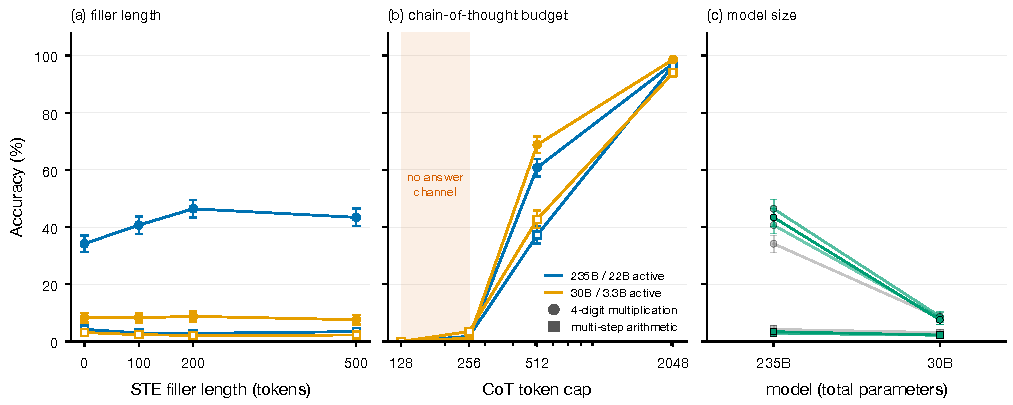
\includegraphics[width=\textwidth]{figs/recovery-sensitivity.pdf}
    \caption{Response curves across the three recovery axes: (a) STE filler
    length, showing inverted-U saturation at 200 tokens on 235B multiplication;
    (b) CoT token cap on a log axis, with the mid-derivation truncation regime
    shaded; (c) model scale from 235B down to 30B under no-CoT conditions.}
    \label{fig:sensitivity}
\end{figure}

\section{Discussion}
\label{sec:discussion}

\paragraph{Parallel width versus serial depth.}
Our results sharpen what prefilled filler tokens compute. On 4-digit
multiplication in Qwen3-235B, ${\sim}200$ semantically inert tokens buy a genuine
$+12.2$~pp at ${\sim}0.6$ extra decode tokens; the same intervention does nothing
on five-step nested arithmetic and nothing on Qwen3-30B at any length. Read
against the expressivity analysis of \citet{pfau2024dot}, this is the signature of
extra parallel attention width applied to circuits the model already has in
nascent form---visible in the $+7.3\pm5.5$~pp scale--filler complementarity---and
not of serial state tracking. For CoT monitorability this yields an empirical
bound rather than a worry: in off-the-shelf models, unmonitored prefill can refine
single-step or parallelisable judgements, but cannot covertly execute deep
multi-step symbolic derivation without training-time adaptation.

\paragraph{Quantization and filler sensitivity.}
Why did our 10-shot multiplication run show $+8.30$~pp where the original found
$-0.4$~pp? Prompting ablations and cache-bypassing re-queries rule out few-shot
formatting, system prompts, and stale responses. Our baseline (58.70\%) sits well
below the original's 69.6\%, while the counting filler restores accuracy to
67.00\%, close to the original's unfilled 69.2\%. That is the pattern of a
precision deficit being partly absorbed by redundant attention over filler
positions, and all our endpoints were FP8. We cannot test the mechanism
internally, since we have no weight-level access to the served model; a controlled
comparison across BF16, FP8 and INT4 checkpoints on identical hardware is the
direct next experiment.

\paragraph{Budget-matched baselines need a truncation floor.}
Taken alone, our efficiency numbers suggest the filler wins at low budget: it cuts
decode reads by $78\times$--$170\times$ and beats token-capped CoT at
$L\leq256$ by more than 45~pp. Tracking answer-cue rates shows that win is a
measurement artefact---a 256-token cap severs the output channel before an answer
exists in over 97\% of trials. Any evaluation of test-time compute, latent
reasoning, or compressed CoT that reports accuracy against a capped baseline
without reporting completion rates is measuring its own parser. The frontier
should also include a smaller model running full CoT, which in our grid is the
point that actually dominates.

\section{Limitations}
\label{sec:limitations}

\begin{itemize}
    \item \textbf{Quantized serving path.} Every available OpenRouter endpoint for
    Qwen3-235B was FP8 during our runs, while the original study's precision is
    unspecified; weight-controlled local deployment is needed to confirm whether
    FP8 explains the 10-shot multiplication divergence.
    \item \textbf{Amortised latency.} Seconds per query are cell completion time
    divided by $N$ at client concurrency 16, not isolated single-stream TTFT and
    TPOT distributions; the ${\sim}16\times$ factor is a throughput ratio and
    carries no per-query interval.
    \item \textbf{Two-point scale estimates.} Parameter derivatives are secant
    slopes across two MoE checkpoints spanning 0.887 decades; intermediate sizes
    could reveal nonlinear capability thresholds, and active- versus
    total-parameter scalings differ by ${\sim}25\%$ because of sparsity.
    \item \textbf{Uncached peak-KV accounting.} Table~\ref{tab:kv} reports
    uncached totals, which is the conservative choice for the filler: its
    0.42$\times$ and 0.37$\times$ ratios already include the full 202-token
    prefix. If a server caches that static prefix once, the filler's unshared KV
    falls to 20.8 and 34.0 tokens---indistinguishable from baseline---so its
    marginal memory cost in production is lower than the table implies, while its
    accuracy ceiling is unchanged.
    \item \textbf{Billed versus visible tokens.} $T_c$ uses OpenRouter billing
    metadata, which slightly exceeds locally re-tokenised visible text (630
    versus 435 tokens for 235B multiplication CoT), so $R_{\mathrm{KV}}$ is an
    upper estimate for CoT.
    \item \textbf{Paired sample.} Headline accuracies and all paired tests use the
    full $N{=}1000$; the per-sample records stored in the results file were
    capped at 200 for size, and we reconstructed the remainder from the response
    cache rather than relying on that cap.
\end{itemize}

\section{Conclusion}
\label{sec:conclusion}

Replicating and extending \citet{baherwani2026not} on Qwen3 models, we find that
prefilled filler tokens unlock a real but tightly circumscribed form of latent
computation. Controlled-vocabulary fillers recover at most ${\sim}19\%$ of full
CoT gains on parallelisable multiplication, confer no benefit on sequential
multi-step arithmetic, saturate at ${\sim}200$ tokens, and vanish on a
$7.7\times$ smaller model. Their $78\times$--$170\times$ decode-read reduction
becomes an accuracy win over budget-matched CoT only while CoT is truncated before
emitting an answer; once CoT has enough budget to finish a derivation, running it
on the smaller model dominates the filler on the larger one in both accuracy and
memory.

Three directions follow. First, mechanistic work across BF16 and FP8 weights
should test whether filler attention compensates for quantization noise in
parallel arithmetic circuits, which would turn our serving-path hypothesis into a
measurement. Second, budget-aware prompting---instructing a CoT model to
summarise and emit an answer before its cap---would test whether the truncation
cliff is a property of the cap or of the prompt, and would make capped CoT a
usable low-budget baseline. Third, safety monitoring for hidden reasoning should
concentrate on RL-trained thinking models rather than static prefill sequences:
our grid bounds what prefill can do without training, and the bound is small.

\section*{Acknowledgments}
Experiments in this work were run and tracked with
OpenResearch~\citep{openresearch}.

\appendix
\section{The ASD-STE100 filler string}
\label{app:filler}

The \texttt{ste\_filler} condition prefills the following 198-word sequence
(199 \texttt{o200k} tokens) verbatim before the answer cue, identically for every
query and every problem:

\begin{quote}\footnotesize\ttfamily\raggedright\sloppy
a an the and or but if then when where which who what why how this that these
those all any both each every some no not only also again always never often
sometimes before after above below between during through about against into
over under up down out off on in at by for with without adjust align apply
assemble attach balance bleed check clean close connect cut decrease disconnect
do examine fill fit fix hold increase insert inspect install keep lift limit
loosen maintain make measure move open operate position pull push put read
remove repair replace rotate run secure select set slow start stop support
tighten turn use verify wait watch bearing bracket clamp clip connector cylinder
diaphragm disc drain filter fluid gauge hose indicator line liquid nut oil part
pipe plug pressure pump screw seal surface system tank test tool valve wire
\end{quote}

The \texttt{ste\_100} and \texttt{ste\_500} conditions use the same stream
truncated to the calibrated token counts. The string is produced by
\texttt{build\_filler("ste\_dictionary", 200, tokenizer)} in the released
harness, so it can be regenerated exactly rather than copied by hand.

\begin{thebibliography}{9}

\bibitem[Baherwani et~al.(2026)]{baherwani2026not}
Vatsal Baherwani, Tom Goldstein, and Ashwinee Panda.
\newblock Not all {LLM} reasoning is visible in the chain-of-thought.
\newblock \emph{arXiv preprint arXiv:2607.22925}, 2026.
\newblock \url{https://arxiv.org/abs/2607.22925}

\bibitem[Damani et~al.(2025)]{damani2025learning}
Mehul Damani, Idan Shenfeld, Andi Peng, Andreea Bobu, and Jacob Andreas.
\newblock Learning how hard to think: Input-adaptive allocation of {LM}
computation.
\newblock In \emph{International Conference on Learning Representations
(ICLR)}, 2025.

\bibitem[Goyal et~al.(2024)]{goyal2024pause}
Sachin Goyal, Ziwei Ji, Ankit~Singh Rawat, Aditya~Krishna Menon, Sanjiv Kumar,
and Vaishnavh Nagarajan.
\newblock Think before you speak: Training language models with pause tokens.
\newblock In \emph{International Conference on Learning Representations
(ICLR)}, 2024.

\bibitem[Pfau et~al.(2024)]{pfau2024dot}
Jacob Pfau, William Merrill, and Samuel~R. Bowman.
\newblock Let's think dot by dot: Hidden computation in transformer language
models.
\newblock In \emph{Conference on Language Modeling (COLM)}, 2024.

\bibitem[Wei et~al.(2022)]{wei2022cot}
Jason Wei, Yi~Tay, Rishi Bommasani, Colin Raffel, Barret Zoph, Sebastian
Borgeaud, Dani Yogatama, Maarten Bosma, Denny Zhou, Donald Metzler, Ed~H. Chi,
Tatsunori Hashimoto, Oriol Vinyals, Percy Liang, Jeff Dean, and William
Fedoruk.
\newblock Chain-of-thought prompting elicits reasoning in large language
models.
\newblock In \emph{Advances in Neural Information Processing Systems
(NeurIPS)}, 2022.

\bibitem[OpenRouter(2026)]{openrouter2026}
OpenRouter.
\newblock OpenRouter: A unified API for {LLM} serving.
\newblock \url{https://openrouter.ai}, 2026. Accessed November 2026.

\bibitem[alphaXiv(2026)]{openresearch}
alphaXiv.
\newblock OpenResearch: The local-first harness and workspace for research
agents.
\newblock \url{https://github.com/alphaXiv/OpenResearch}, 2026.

\end{thebibliography}

\end{document}
